%%%%%%%%%%%%%%%%%%%%%%%%%%%%%%%%%%%%%%%%%%%%%%%%%%%%%%%%%%%%%%%%
% %
% Due Date %
% Andrew Gibson %
% ECE 351 lab, Section 53 %
% Lab 9 %
% Due 28 Mar 2023 %
% Fast Fourier Transform %
% https://github.com/gibs0630/ECE351\_Code %
% https://github.com/gibs0630/ECE351\_Reports %
% %
%%%%%%%%%%%%%%%%%%%%%%%%%%%%%%%%%%%%%%%%%%%%%%%%%%%%%%%%%%%%%%%%

\documentclass[12pt,a4paper]{article}
\usepackage[utf8]{inputenc}
\usepackage[greek,english]{babel}
\usepackage{alphabeta} 
\usepackage[pdftex]{graphicx}
\usepackage[top=1in, bottom=1in, left=1in, right=1in]{geometry}
\linespread{1.06}
\setlength{\parskip}{8pt plus2pt minus2pt}
\widowpenalty 10000
\clubpenalty 10000
\newcommand{\eat}[1]{}
\newcommand{\HRule}{\rule{\linewidth}{0.5mm}}
\usepackage[official]{eurosym}
\usepackage{enumitem}
\setlist{nolistsep,noitemsep}
\usepackage[hidelinks]{hyperref}
\usepackage{cite}
\usepackage{lipsum}

\newcommand{\Q}{\leavevmode\par\textbf {Q:}}
\newcommand{\A}{\par\textbf{A:} \normalfont}

\hypersetup{colorlinks=true, linkcolor=black, urlcolor=blue}

\begin{document}
%===========================================================
\begin{titlepage}
\begin{center}
% Top 
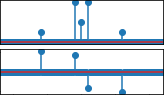
\includegraphics[width=0.55\textwidth]{titlepage_image.png}~\\[2cm]
% Title
\HRule \\[0.4cm]
{ \LARGE 
  \textbf{Project Report for ECE 351}\\[0.4cm]
  \emph{Lab 9: Fast Fourier Transform}\\[0.4cm]
}
\HRule \\[1.5cm]
% Author
{ \large
  Andrew Gibson \\[0.1cm]
 28 March 2023\\[0.1cm]
  \url{https://github.com/gibs0630/ECE351\_Code}\\[0.1cm]
  \url{https://github.com/gibs0630/ECE351\_Reports}\\[0.1cm]
  %#\texttt{user@cut.ac.cy}
}
\vfill
%\textsc{\Large Cyprus University of Technology}\\[0.4cm]\textsc{\large Department of Electrical Engineering,\\Computer Engineering \& Informatics}\\[0.4cm]
% Bottom
{\large }
 
\end{center}
\end{titlepage}
%\begin{abstract}
%\lipsum[1-2]
%\addtocontents{toc}{\protect\thispagestyle{empty}}
%\end{abstract}
\newpage
%===========================================================
\tableofcontents
\addtocontents{toc}{\protect\thispagestyle{empty}}
\newpage
\setcounter{page}{1}
%===========================================================
%===========================================================
\section{Introduction}\label{sec:intro}
With Python, it is possible to create a Fourier signal analyses.  Being able to present the analysis is important to quickly catch important information at a glance.

\section{Equations}\label{sec:lit-rev}
Formula's used
unit step function
\[
u(x) = \left\{
        \begin{array}{ll}
            0 & \quad t < 0 \\
            1 & \quad t \geq 0
        \end{array}
    \right.
\]
pulse function

\[P_{\tau} = u \left (t-\frac \tau 2 \right)-u \left (t+\frac \tau 2 \right)\]

Fourier's series
\[x(t) = \frac 1  2 a_0 + \sum_{k=1}^\infty \left[ a_k cos \left (k \frac {2\pi}  T t \right) + b_k sin \left(k \frac {2\pi}  T t \right) \right]\]

\[a_0 = \frac 2 T \int_0^T \left [ x_0(t) dt \right ]\]

\[a_k = \frac 2 T \int_0^T \left [ x_0(t) cos \left (k \frac {2 \pi} T t \right )dt \right ]\]

\[b_k = \frac 2 T \int_0^T \left [ x_0(t) sin \left (k \frac {2 \pi} T t \right )dt \right ]\]


equations from the lab

\[x_0(t) = 2 P_{\frac T 2} \left (t-\frac T 4 \right)- 1\]
\[a_k =  0\]
\[b_k =   \frac 2  {k \pi}   \left [ 1-(-1)^k \right ] \]


\[x(t) = \frac 2  { \pi }  \sum _{k=1}^\infty \left[ \left (\frac 1  {k}   \left [1- (-1)^k \right ] \right) sin \left(k \frac {2 \pi}  {T} t \right) \right]\]

\[x(t) = \frac 4  { \pi }  \sum_{n=1}^\infty \left[ \left(\frac 1  {2n-1}    \right) sin \left((2n-1) \frac {2 \pi} {T} t \right) \right]\]


\section{Methodology}\label{sec:meth}
This lab had us create a presentation of various signals using Fourier series. We used Python to create a function that performs a Fourier series (using few libraries to do the heavy lifting of computing the Fourier transform). A function was also created that would generate the plots of the series in a presentable format. The format was to have the original function over time, the magnitude of the Fourier series, phase angle of the Fourier series, zoomed in magnitude of the Fourier series too more clearly see the important magnitudes, and phase angle of the Fourier series with the same zoom level.

\section{Results}\label{sec:res}
\subsection*{Part 1}


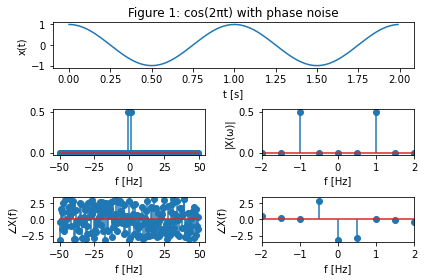
\includegraphics[width=1\textwidth]{Figure1.png}\\
Figure 1 shows the presentation of from the signal where $x(t)=cos(2 \pi t)$, with the angle noise not being suppressed. The phase angle appears erratic because of Boolean algebra with vary small numbers.

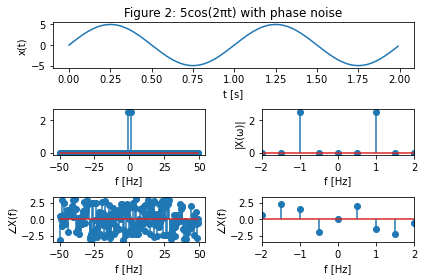
\includegraphics[width=1\textwidth]{Figure2.png}\\
Figure 2 shows the presentation of from the signal where $x(t) =5cos(2 \pi t)$, with the angle noise not being suppressed. The phase angle appears erratic because of Boolean algebra with vary small numbers.

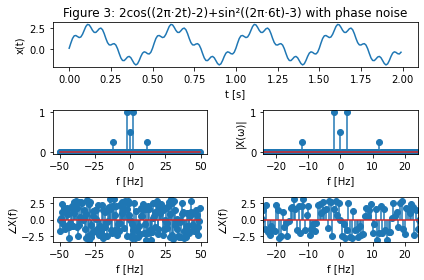
\includegraphics[width=1\textwidth]{Figure3.png}\\
Figure 3 shows the presentation of from the signal where $x(t) =2cos((2 \pi\cdot 2 t)-2)+sin^2((2 \pi\cdot 6 t)-2)$, with the angle noise not being suppressed. The phase angle appears erratic because of Boolean algebra with vary small numbers.

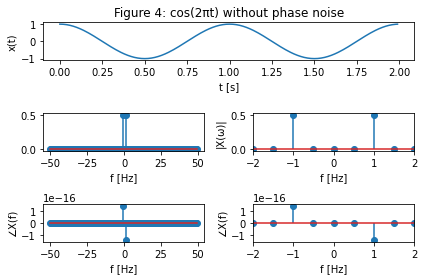
\includegraphics[width=1\textwidth]{Figure4.png}\\
Figure 4 shows the presentation of from the signal where $x(t) =5cos(2 \pi t)$, with the angle noise being removed if the magnitude was less than 1e-10.

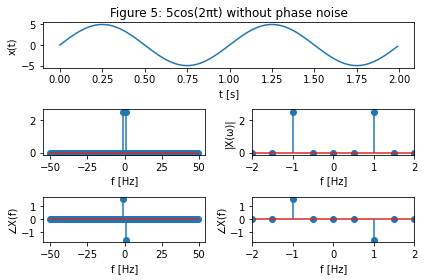
\includegraphics[width=1\textwidth]{Figure5.png}\\
Figure 5 shows the presentation of from the signal where $x(t) =2cos((2 \pi\cdot 2 t)-2)+sin^2((2 \pi\cdot 6 t)-2)$, with the angle noise being removed if the magnitude was less than 1e-10.

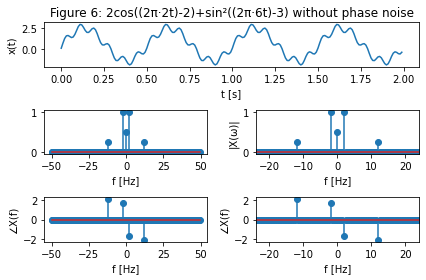
\includegraphics[width=1\textwidth]{Figure6.png}\\
Figure 6 shows the presentation of from the signal where $x(t)=cos(2 \pi t)$, with the angle noise being removed if the magnitude was less than 1e-10.

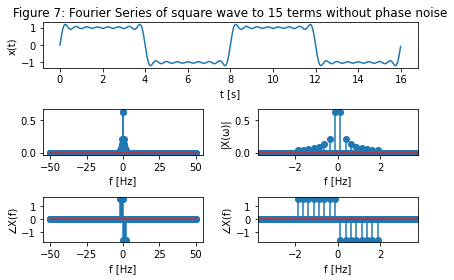
\includegraphics[width=1\textwidth]{Figure7.png}\\
Figure 7 shows the presentation of from the signal created from the first 15 terms of the Fourier Series of a square, with the angle noise being removed if the magnitude was less than 1e-10.




\section{Questions}\label{sec:res}

Q1) What happens if fs is lower? If it is higher? fs in your report must span a few orders of magnitude.
A1) Adjusting fs will change the domain in the Fourier space.  fs is for the sampling frequency, and it would signify the maximum Hertz that data can be gathered.


Q2) What difference does eliminating the small phase magnitudes make?
A2) eliminating the noise in the phase (which is caused by Boolean algebra error when the computer calculates it) allows us to see the phases of the frequencies that have a significant effect.

Q3) Verify your results from Tasks 1 and 2 using the Fourier transforms of cosine and sine. Explain why your results are correct. You will need the transforms in terms of Hz, not rad/s. For example, the Fourier transform of cosine (in Hz) is:
\[\mathcal{F} {cos(2 \pi f_t)} = 1/2 [\delta(f-f_0)+\delta(f+f_0)]\]
A3)from task 1, there are 0.5 tall spikes at -1 and 1, and the phases at -1 and 1 are 0.
\[0.5 \delta(f+1)+ 0.5 \delta(f-1) = 0.5 [\delta(f=1)+\delta(f-1)] = \mathcal{F}{cos(2 \pi 1)}\]


from task 2, there are 2.5 tall spikes at -1 and 1, and the phases are at about 1.5 and -1.5 respectively (1.5 is approximately $\pi$/2)
\[2.5 j \delta(f+1) - 2.5 j \delta(f-1) = j2.5 [\delta(f+1)-\delta(f-1)] = \mathcal{F}{5sin(2 \pi 1)}\]


Q5) Leave any feedback on the clarity of lab tasks, expectations, and deliverables.
A5) This lab was pretty strait forward, other than "figure out how to code the presentation plot".  I had to learn about Axes and Subplots to get it to present right.
Also, Question 3 wants us to  verify results from Task 1 and 2, which sure could be done, but with the phase noise, it was slightly confusing even though only the phase at the specific locations are used.



\section{Conclusion}\label{sec:res}
When conducting analysis, it is important to be able to present the findings.  sometimes those finding are hidden behind noise because of a too wide of a viewed domain or because of error caused by the inherit nature of the computers.



%\lipsum[7-8]\cite{knuthwebsite}
%===========================================================
%===========================================================
\bibliographystyle{ieeetr}
\bibliography{refs}
\end{document} 
Annotations











